% Title:
% 	Presentation template
% ----------------------
% Description:
% 	A clean, sans-serif presentation template.
%   This presentation uses custom fonts. You need to compile with xelatex,
%   and download Open Sans and Ubuntu Mono from:
%	
%	- https://www.fontsquirrel.com/fonts/open-sans
%	- https://www.fontsquirrel.com/fonts/ubuntu-mono
%
% Creator: Tommy Odland

% -------------------------------------------------------------------------
% Setup
% -------------------------------------------------------------------------
% Options for aspectratio: 1610, 149, 54, 43 and 32, 169
\documentclass[12pt, aspectratio=149]{beamer}
\usepackage[utf8]{inputenc}
\usepackage[english]{babel}% Alternatives: 'norsk', 'english'
\usepackage[expansion=false]{microtype}% Fixes to make typography better
\usecolortheme{beaver} % Decent options: beaver, rose, crane
%\useoutertheme{split}
%\useoutertheme[footline=authortitle]{miniframes}
\usepackage{listings}% To include source-code
\usepackage{booktabs}% Professional tables
\usepackage{multirow}
\usepackage{xcolor}

% https://tex.stackexchange.com/questions/159667/including-python-code-in-beamer
% https://ftp.eq.uc.pt/software/TeX/macros/latex/contrib/minted/minted.pdf
\usepackage{minted}

% Title information common to every file
\institute{Equinor}
\date{Edited: \today}
\author{Tommy Odland \and Knut Utne Hollund}

% -------------------------------------------------------------------------
% Package imports
% -------------------------------------------------------------------------
\usepackage{etoolbox}
\usepackage{graphicx}
\usepackage{tikz}
\usepackage{amsmath,amsthm,amsfonts,amssymb,mathtools, bm}
\usepackage{hyperref}
\usepackage{listings}
\usepackage[sharp]{easylist}
\usepackage{multicol}
\usepackage{tikz-cd}

\usepackage[absolute,overlay]{textpos}
\setbeamertemplate{footline}[frame number]  
\usepackage{graphbox}

\newcommand{\norm}[1]{\left\lVert#1\right\rVert}

\setbeamertemplate{footline}{%
%	\includegraphics[align=c, height=0.5cm]{figs/sonat_logo_color.png}%
	\hfill%
	\usebeamercolor[fg]{page number in head/foot}%
%	\usebeamerfont{page number in head/foot}%
%	\insertframenumber\,/\,\inserttotalframenumber\kern1em%
}

% Set the math fonts - should be set before the others fonts, not sure why
\usepackage{sansmath} % Enables turning on sans-serif math mode
% \sansmath % Enable sans-serif math for rest of document

% Set fonts to Open Sans and Ubuntu mono
\usefonttheme{professionalfonts}
\usepackage{fontspec}
\setmainfont{Open Sans}
\setsansfont{Open Sans}
\setmonofont{Ubuntu Mono}
\usefonttheme{serif}

%gets rid of bottom navigation symbols
\setbeamertemplate{navigation symbols}{}

% Set up colors to be used
\definecolor{titlecolor}{RGB}{128,54,63}
\definecolor{bggray}{RGB}{242,242,242}
\definecolor{bggraydark}{RGB}{217,217,217}

% Change the default colors
\setbeamercolor*{title}{bg=bggray,fg=titlecolor}
\AtBeginEnvironment{theorem}{%
	\setbeamercolor{block title}{fg=titlecolor, bg=bggraydark}
	\setbeamercolor{block body}{fg=black,bg=bggray}
}
\AtBeginEnvironment{proof}{%
	\setbeamercolor{block title}{fg=titlecolor, bg=bggraydark}
	\setbeamercolor{block body}{fg=black,bg=bggray}
}
\AtBeginEnvironment{example}{%
	\setbeamercolor{block title example}{bg=bggraydark}
	\setbeamercolor{block body example}{fg=black,bg=bggray}
}
\AtBeginEnvironment{definition}{%
	\setbeamercolor{block title}{bg=bggraydark}
	\setbeamercolor{block body}{fg=black,bg=bggray}
}

\setbeamercolor{block title example}{bg=bggraydark}
\setbeamercolor{block body example}{fg=black,bg=bggray}
\setbeamercolor{block title}{fg=titlecolor, bg=bggraydark}
\setbeamercolor{block body}{fg=black,bg=bggray}

\setbeamercolor{frametitle}{fg=titlecolor,bg=bggray}
\setbeamercolor{section in head/foot}{bg=black}
\setbeamercolor{author in head/foot}{bg=black}
\setbeamercolor{date in head/foot}{fg=titlecolor}

% Spacing for lists
\newcommand{\listSpace}{0.2em}

% Theorems, equations, definitions setup
\theoremstyle{plain}

% Slides for sections
\AtBeginSection[]{
	\begin{frame}
		\vfill
		\centering
		\begin{beamercolorbox}[sep=8pt,center,shadow=false,rounded=false]{title}
			\usebeamerfont{title}\insertsectionhead\par%
		\end{beamercolorbox}
		\vfill
	\end{frame}
}

% Title information
\title{Wanna see my collection of random numbers?}
\subtitle{Course overview}

% -------------------------------------------------------------------------
% Document start
% -------------------------------------------------------------------------
\begin{document}

\begin{frame}{}
	\begin{center}
			\vfill
	{\huge Wanna see my collection of random numbers?}
	\vfill
	{\large Clever subtitle here}
	\vfill
	%\includegraphics[width=0.7\linewidth]{figs/best_party}
	
	% \includegraphics[width=0.7\linewidth]{figs/optimizeem}

	\vfill
	{\large  Tommy Odland and Knut Utne Hollund}
	\vfill
	{\small \texttt{https://github.com/tommyod/rng}}
	\vfill
	\today
	\vfill
	\end{center}
\end{frame}


\begin{frame}[fragile]{Agenda}
	\begin{center}
		% \includegraphics[width=0.7\linewidth]{figs/best_party}
	\end{center}
	
	\begin{easylist}[itemize]
		# \textbf{Modeling}: Define what we mean by a good party
		# \textbf{Computing}: Learn how to find the best party efficiently
		## $\binom{151}{6} = 14\,888\,600\,755$ possible parties
		## Checking every possible party takes $\approx 5$ days
		# \textbf{Inspection}: Evaluate party using Shapley values
	\end{easylist}
\end{frame}

% ==================================================================================
\section{Introduction}


\begin{frame}[fragile]{Probability Density Functions (PDFs)}
\begin{columns}
\begin{column}{0.5\textwidth}
    \begin{center}
     \begin{figure}
     	\centering
     	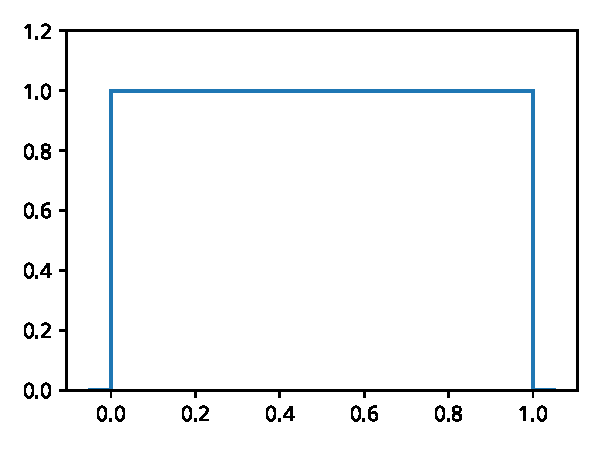
\includegraphics[width=0.99\linewidth]{figures/uniform}
     \end{figure}
     \begin{minted}{pycon}
>>> import random
>>> random.random()
0.9757805031464292
     \end{minted}
     \end{center}
\end{column}
\begin{column}{0.5\textwidth}  %%<--- here
    \begin{center}
     \begin{figure}
     	\centering
     	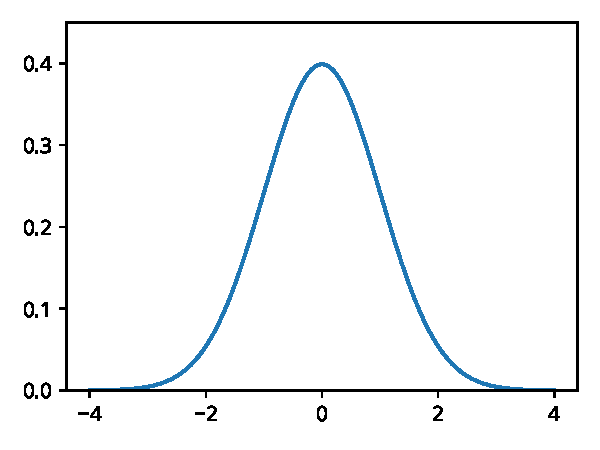
\includegraphics[width=0.99\linewidth]{figures/normal}
     \end{figure}
      \begin{minted}{pycon}
>>> import random
>>> random.gauss(0, 1)
-0.19223758016631237
      \end{minted}
     \end{center}
\end{column}
\end{columns}
\end{frame}

\begin{frame}[fragile]{Sampling PDFs}
\begin{columns}
\begin{column}{0.5\textwidth}
    \begin{center}
     \begin{figure}
     	\centering
     	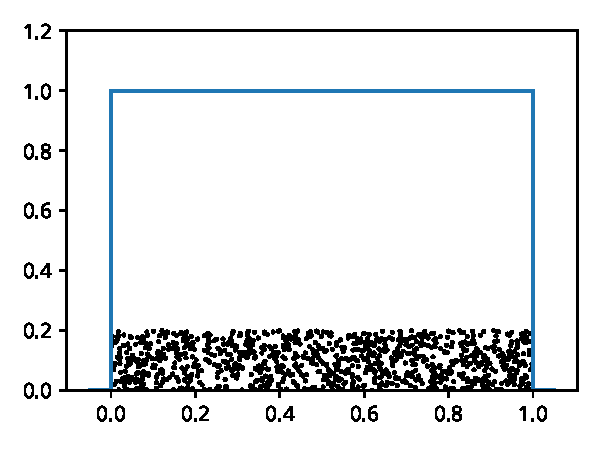
\includegraphics[width=0.99\linewidth]{figures/uniform_samples}
     \end{figure}
     \begin{minted}{pycon}
>>> import random
>>> random.random()
0.9757805031464292
     \end{minted}
     \end{center}
\end{column}
\begin{column}{0.5\textwidth}  %%<--- here
    \begin{center}
     \begin{figure}
     	\centering
     	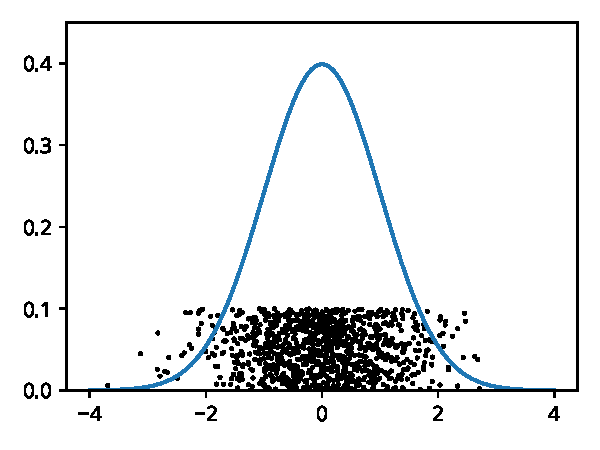
\includegraphics[width=0.99\linewidth]{figures/normal_samples}
     \end{figure}
      \begin{minted}{pycon}
>>> import random
>>> random.gauss(0, 1)
-0.19223758016631237
      \end{minted}
     \end{center}
\end{column}
\end{columns}
\end{frame}

\begin{frame}[fragile]{Using samples to generate histograms}
\begin{columns}
\begin{column}{0.5\textwidth}
    \begin{center}
     \begin{figure}
     	\centering
     	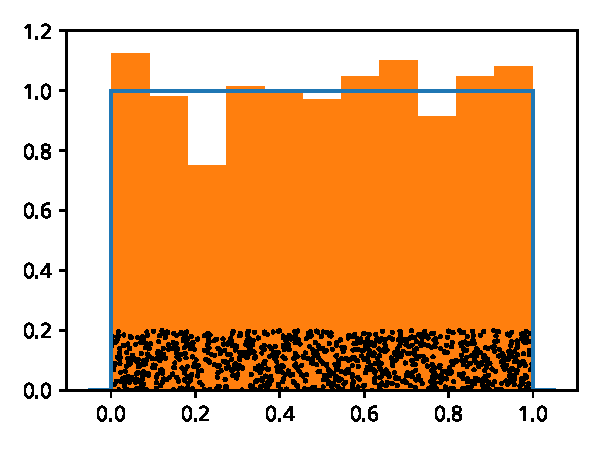
\includegraphics[width=0.99\linewidth]{figures/uniform_samples_hist}
     \end{figure}
     \begin{minted}{pycon}
>>> import random
>>> random.random()
0.9757805031464292
     \end{minted}
     \end{center}
\end{column}
\begin{column}{0.5\textwidth}  %%<--- here
    \begin{center}
     \begin{figure}
     	\centering
     	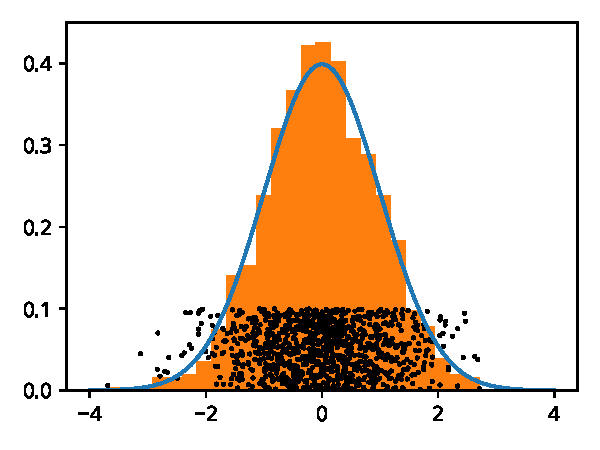
\includegraphics[width=0.99\linewidth]{figures/normal_samples_hist}
     \end{figure}
      \begin{minted}{pycon}
>>> import random
>>> random.gauss(0, 1)
-0.19223758016631237
      \end{minted}
     \end{center}
\end{column}
\end{columns}
\end{frame}

\section{Monte Carlo}

\begin{frame}[fragile]{Mutual fund}
\begin{columns}
\begin{column}{0.55\textwidth}
    \begin{center}
     \begin{minted}[fontsize=\footnotesize]{python3} 


def simulate(years, yearly, interest):
    saved = 0
    yield saved
    for year in range(years):
        saved = saved * interest + yearly
        yield saved
        
years = 18
yearly = 12
interest = 1.05

list(simulate(years, yearly, interest))
     \end{minted}
     \end{center}
\end{column}
\begin{column}{0.45\textwidth}  %%<--- here
    \begin{center}
     \begin{figure}
     	\centering
     	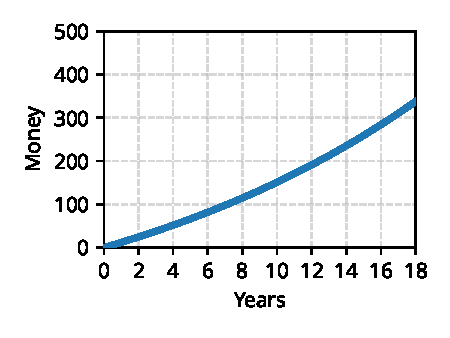
\includegraphics[width=0.99\linewidth]{figures/mutual_fund}
     \end{figure}
     \end{center}
\end{column}
\end{columns}
\end{frame}

\begin{frame}[fragile]{Mutual fund}
\begin{columns}
\begin{column}{0.55\textwidth}
    \begin{center}
     \begin{minted}[fontsize=\footnotesize]{python3} 
import random

def simulate_rng(years, yearly, interest):
    saved = 0
    yield saved
    for year in range(years):
        ir = random.gauss(*interest)
        saved = saved * ir + yearly
        yield saved
        
years = 18
yearly = 12
interest = (1.05, 0.1)

list(simulate_rng(years, yearly, interest))
     \end{minted}
     \end{center}
\end{column}
\begin{column}{0.45\textwidth}  %%<--- here
    \begin{center}
     \begin{figure}
     	\centering
     	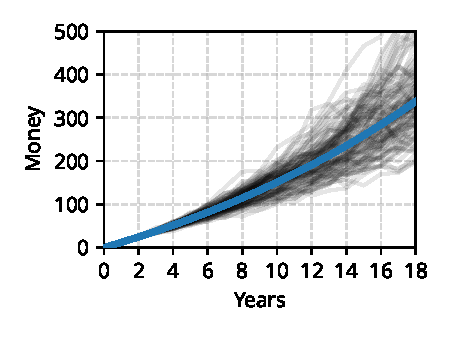
\includegraphics[width=0.99\linewidth]{figures/mutual_fund_simulations}
     \end{figure}
     \end{center}
\end{column}
\end{columns}
\end{frame}

\begin{frame}[fragile]{A simple idea: top stats}
\begin{figure}
	\centering
	% \includegraphics[width=0.7\linewidth]{figs/best_stats_party}
	\begin{center}
		\textbf{Disadvantage: ignores type information}
	\end{center}
\end{figure}
\end{frame}

\begin{frame}[fragile]{Optimization problem}
	More formally, we want to solve:
	\\
	\begin{align*}
	& \text{maximize}   && 
	\left(
	\operatorname{geom\_avg}_j \left( \text{BEST EDGE}_j \right) ,
	\sum_i \operatorname{total\_stats}_i \, x_i
	\right)
	\\
	& \text{subject to} && \text{BEST EDGE}_j= \max_i \left( \text{edge}(i, j) \, x_i \right) \quad \forall \, j \\
	& && \sum_i x_i = 6    \\
	& && x_{i} \in \{0, 1\}   \\
& && 	\text{BEST EDGE}_j \in \mathbb{R}_+  
	\end{align*}
\end{frame}


\section{Resampling}

\begin{frame}[fragile]{Groceries}
\begin{columns}
\begin{column}{0.50\textwidth}
    \begin{center}
     \begin{minted}[fontsize=\footnotesize]{pycon} 
>>> money_per_day
array([0, 0, 471.9, 784.22,0,  ...])
>>> money_per_day.sum()
8911.18
     \end{minted}
     \end{center}	
\end{column}
\begin{column}{0.50\textwidth}  %%<--- here
    \begin{center}
     \begin{figure}
     	\centering
     	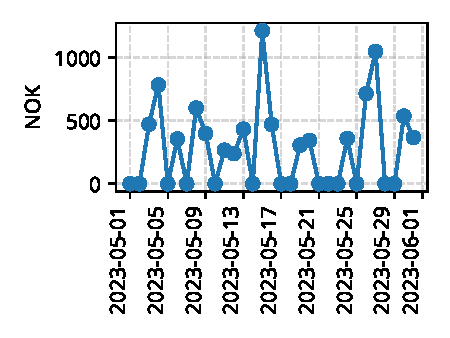
\includegraphics[width=0.99\linewidth]{figures/groceries_data}
     \end{figure}
     \end{center}
\end{column}
\end{columns}
\end{frame}

\begin{frame}[fragile]{Groceries}
\begin{center}
 \begin{figure}
    	\centering
    	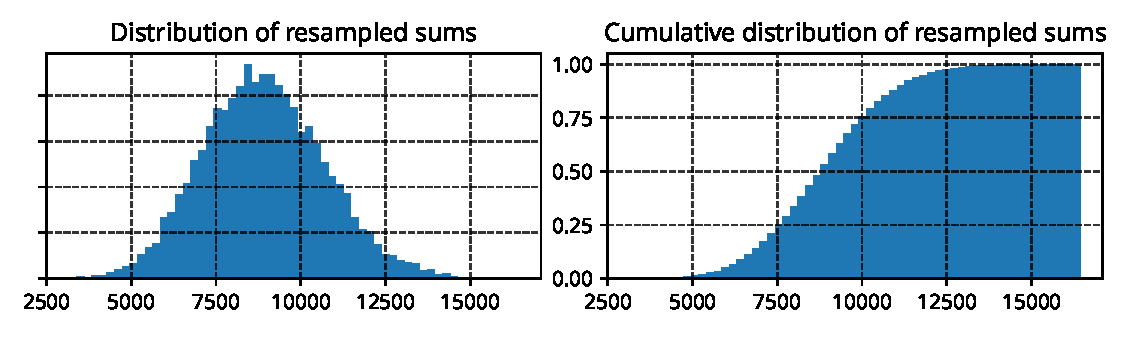
\includegraphics[width=0.99\linewidth]{figures/groceries_data_resampled}
 \end{figure}
 \end{center}

\begin{center}
\begin{minted}[fontsize=\footnotesize]{python3} 
import numpy as np
import matplotlib.pyplot as plt

resamples = np.random.choice(money_per_day, 
            size=(9999, len(money_per_day)), 
            replace=True)

plt.hist(resamples.sum(axis=1), bins="auto", 
         density=True, cumulative=True)
\end{minted}
\end{center}
     
\end{frame}


\begin{frame}[fragile]{Approaches}
	
\begin{minted}{python3}
import numpy as np
    
def incmatrix(genl1,genl2):
    m = len(genl1)
    n = len(genl2)
    M = None #to become the incidence matrix
    VT = np.zeros((n*m,1), int)  #dummy variable

    for i in range(m-1):
        for j in range(i+1, m):
            [r,c] = np.where(M2 == M1[i,j])
    return M
\end{minted}
\end{frame}


% ==================================================================================
\section{Computing}


\begin{frame}[fragile]{Greedy algorithm}
	
\begin{figure}
	\centering
	% \includegraphics[width=0.7\linewidth]{figs/greedy_party}
\end{figure}
	
\begin{easylist}[itemize]
	# Start with an empty party $P := \{\}$
	# while $|P| < 6$ do:
	## go through every non-chosen candiate $c$
	### evaluate the resulting party $P \cup c$
	## select the best non-chosen candidate pokemon $c^\star$
	## add this Pokémon to the party: $P := P \cup c$
\end{easylist}
\vspace*{1em}
Complexity: $151 + 150 + \cdots + 146 = 891$ evaluations
\end{frame}

\end{document}
